% !TeX program = xelatex

\documentclass[aspectratio=169]{beamer}
\usetheme[progressbar=frametitle,numbering=fraction,sectionpage=none]{metropolis}           % Use metropolis theme
\usepackage[sorting=none,natbib=true,backend=biber,citestyle=authoryear,style=numeric,datamodel=applicabledoc,defernumbers=true]{biblatex}
\graphicspath{{media}}

\title{\LaTeX~tips and tricks}
\subtitle{SpaSys lunch talk}
\date{Wednesday 2022-09-27}
\author{Konstantinos Kanavouras}
\institute{University of Luxembourg}
\titlegraphic{\hfill\includegraphics[height=1.5cm]{SnT_UL_colour_logo.png}}

\usepackage{array}

%\usepackage{polyglossia}
\usepackage{csquotes}
\usepackage{graphicx}
\usepackage{colortbl}
\usepackage{minted}
\usepackage[inline]{enumitem}
\usepackage{relsize}
\usepackage{ragged2e}
\usepackage{multirow}
\usepackage{tcolorbox}
\usepackage{gensymb}
\usepackage{tikz}
\usepackage{multicol}
\usepackage{siunitx}
\usepackage{subcaption}
\usepackage{xcolor-material}
\usepackage{listings}
\usepackage{pdflscape}
\usepackage[nameinlink]{cleveref}
\tcbuselibrary{skins,xparse,breakable}


\newtcbox{\todo}{on line,colback=red!5!white,colframe=red!75!black,coltitle=red!75!black,fonttitle=\bfseries,fontupper=\footnotesize,title=TODO,detach title,before upper={\tcbtitle\ },nobeforeafter,tcbox raise base,top=0pt,bottom=0pt,left=0mm,right=0mm,toprule=0mm,bottomrule=0mm,boxsep=0.7mm,}

%\RecustomVerbatimEnvironment{Verbatim}{BVerbatim}{}

\definecolor{nonex}{HTML}{cc4422}
\definecolor{corex}{HTML}{22dd55}

%\usepackage{xgreek}
%\setdefaultlanguage{english}
%\setotherlanguage{greek}

\newcolumntype{Z}{>{\centering\arraybackslash\hspace{0pt}}X}%% right 
\newcolumntype{Y}{>{\RaggedLeft\arraybackslash\hspace{0pt}}X}%% left 
\newcolumntype{W}{>{\RaggedRight\arraybackslash\hspace{0pt}}X}%% lef
\newcolumntype{L}[1]{>{\RaggedRight\arraybackslash\hspace{0pt}}p{#1}}%% right
\newcolumntype{R}[1]{>{\RaggedLeft\arraybackslash\hspace{0pt}}p{#1}}%% centered
\newcolumntype{C}[1]{>{\Centering\arraybackslash\hspace{0pt}}p{#1}}

\AtBeginSection[]
{
    \begin{frame}
        \frametitle{\secname}
        \begin{multicols}{2}
        \tableofcontents[currentsection]
        \end{multicols}
    \end{frame}
}

\AtBeginSubsection[]
{
	\begin{frame}
		\frametitle{\secname~\textemdash~\subsecname}
		\begin{multicols}{2}
			\tableofcontents[currentsubsection]
		\end{multicols}
	\end{frame}
}

% [x] Tips for writing
%  [x] technical writing tips
%  [x] afroditi picture
%  [x] text vs variables
%  [X] punctuation
%  [x] export images as PDF
% [ ] Overleaf (project, review)
% [ ] Introductory parts of the tamplate
% [x] Bibliography
%   [x] .bib and how to find citations
%   [x] standards CCSDS & ECSS
%   [x] applicable docs
% [x] Tables
%   [x] websites
%   [x] column types
%   [x] tablestyles
%   [x] multicolumn/multirow
% [x] Acronyms
% [x] Requirements
% [x] Confidential stuff
% [x] Positioning
%  [x] htb H κλπ
% [x] autoref


\usepackage{fontspec}
\newfontfamily\examplefont[Script=Latin,Ligatures=TeX]{Droid Serif}

\usepackage{minted}
\usepackage{etoolbox}
\AtBeginEnvironment{minted}{\fontsize{10}{10}\selectfont}

\usepackage{mathtools}

\usepackage[normalem]{ulem}

\usepackage{environ}
\NewEnviron{lex}{%
        \colorbox{white}{\hspace{1ex}\parbox{.8\columnwidth}{\examplefont\vspace{1ex}%
                        \BODY
        \vspace{1ex}}\hspace{1ex}}%
}

\setitemize{label=\usebeamerfont*{itemize item}%
  \usebeamercolor[fg]{itemize item}
  \usebeamertemplate{itemize item}}


\metroset{block=fill}


\definecolor{sntRed}{RGB}{228,30,10}
\definecolor{sntPurple}{RGB}{88,31,126}
\definecolor{sntCyan}{RGB}{0,150,215}

%\definecolor{mDarkBrown}{RGB}{228,30,10}
%\definecolor{mDarkTeal}{RGB}{88,31,126}
%\definecolor{mLightBrown}{RGB}{228,30,10}
%\definecolor{mLightGreen}{RGB}{0,150,215}

\setbeamertemplate{mini frame}{}
\setbeamertemplate{mini frame in current section}{}
\setbeamertemplate{mini frame in current subsection}{}
\setbeamercolor{normal text}{fg=sntCyan!30!black}
\setbeamercolor{structure}{fg=sntPurple, bg=sntPurple}
\setbeamercolor{section in head/foot}{fg=normal text.bg, bg=structure.fg}
\setbeamercolor{subsection in head/foot}{fg=normal text.bg, bg=structure.fg}
\setbeamercolor{progress bar}{fg=sntRed, bg=sntRed}
\makeatletter
\setbeamertemplate{footline}{%
        \begin{beamercolorbox}[colsep=1.5pt]{upper separation line head}
        \end{beamercolorbox}
        \begin{beamercolorbox}{section in head/foot}
                \insertsectionnavigationhorizontal{.95\paperwidth}{}{\hskip0pt plus1filll}%
                \hfil
                \textcolor{gray}{\insertframenumber}\hspace*{.2ex}%
                \vskip3pt%
        \end{beamercolorbox}%
        \begin{beamercolorbox}[colsep=1.5pt]{lower separation line head}
        \end{beamercolorbox}
}
\makeatother

\begin{document}
 \maketitle
	

	

    \begin{frame}
    	\centering
    	
    	\textbf{What is this presentation?}
    	
    	\LaTeX~tips and tricks
    \end{frame}

	{\usebackgroundtemplate{%
		\includegraphics[keepaspectratio,width=\paperwidth]{capybara_cropped}}
	\begin{frame}[standout]{Question}
		
		
		\textbf{Is \LaTeX~a programming language?}
	\end{frame}
	}

	\section{Formatted documents}
	
	\subsection{Images}
	
	 \begin{frame}[fragile]{Image size}
		Use \mintinline{latex}|[width=]| instead of \mintinline{latex}|[scale=]| for images!
		\vspace{4mm}
		\begin{example}
			\vspace*{2mm}
				\begin{minted}[numbersep=5pt,fontsize=\small]{latex}
  \begin{figure}[h]
    \centering
    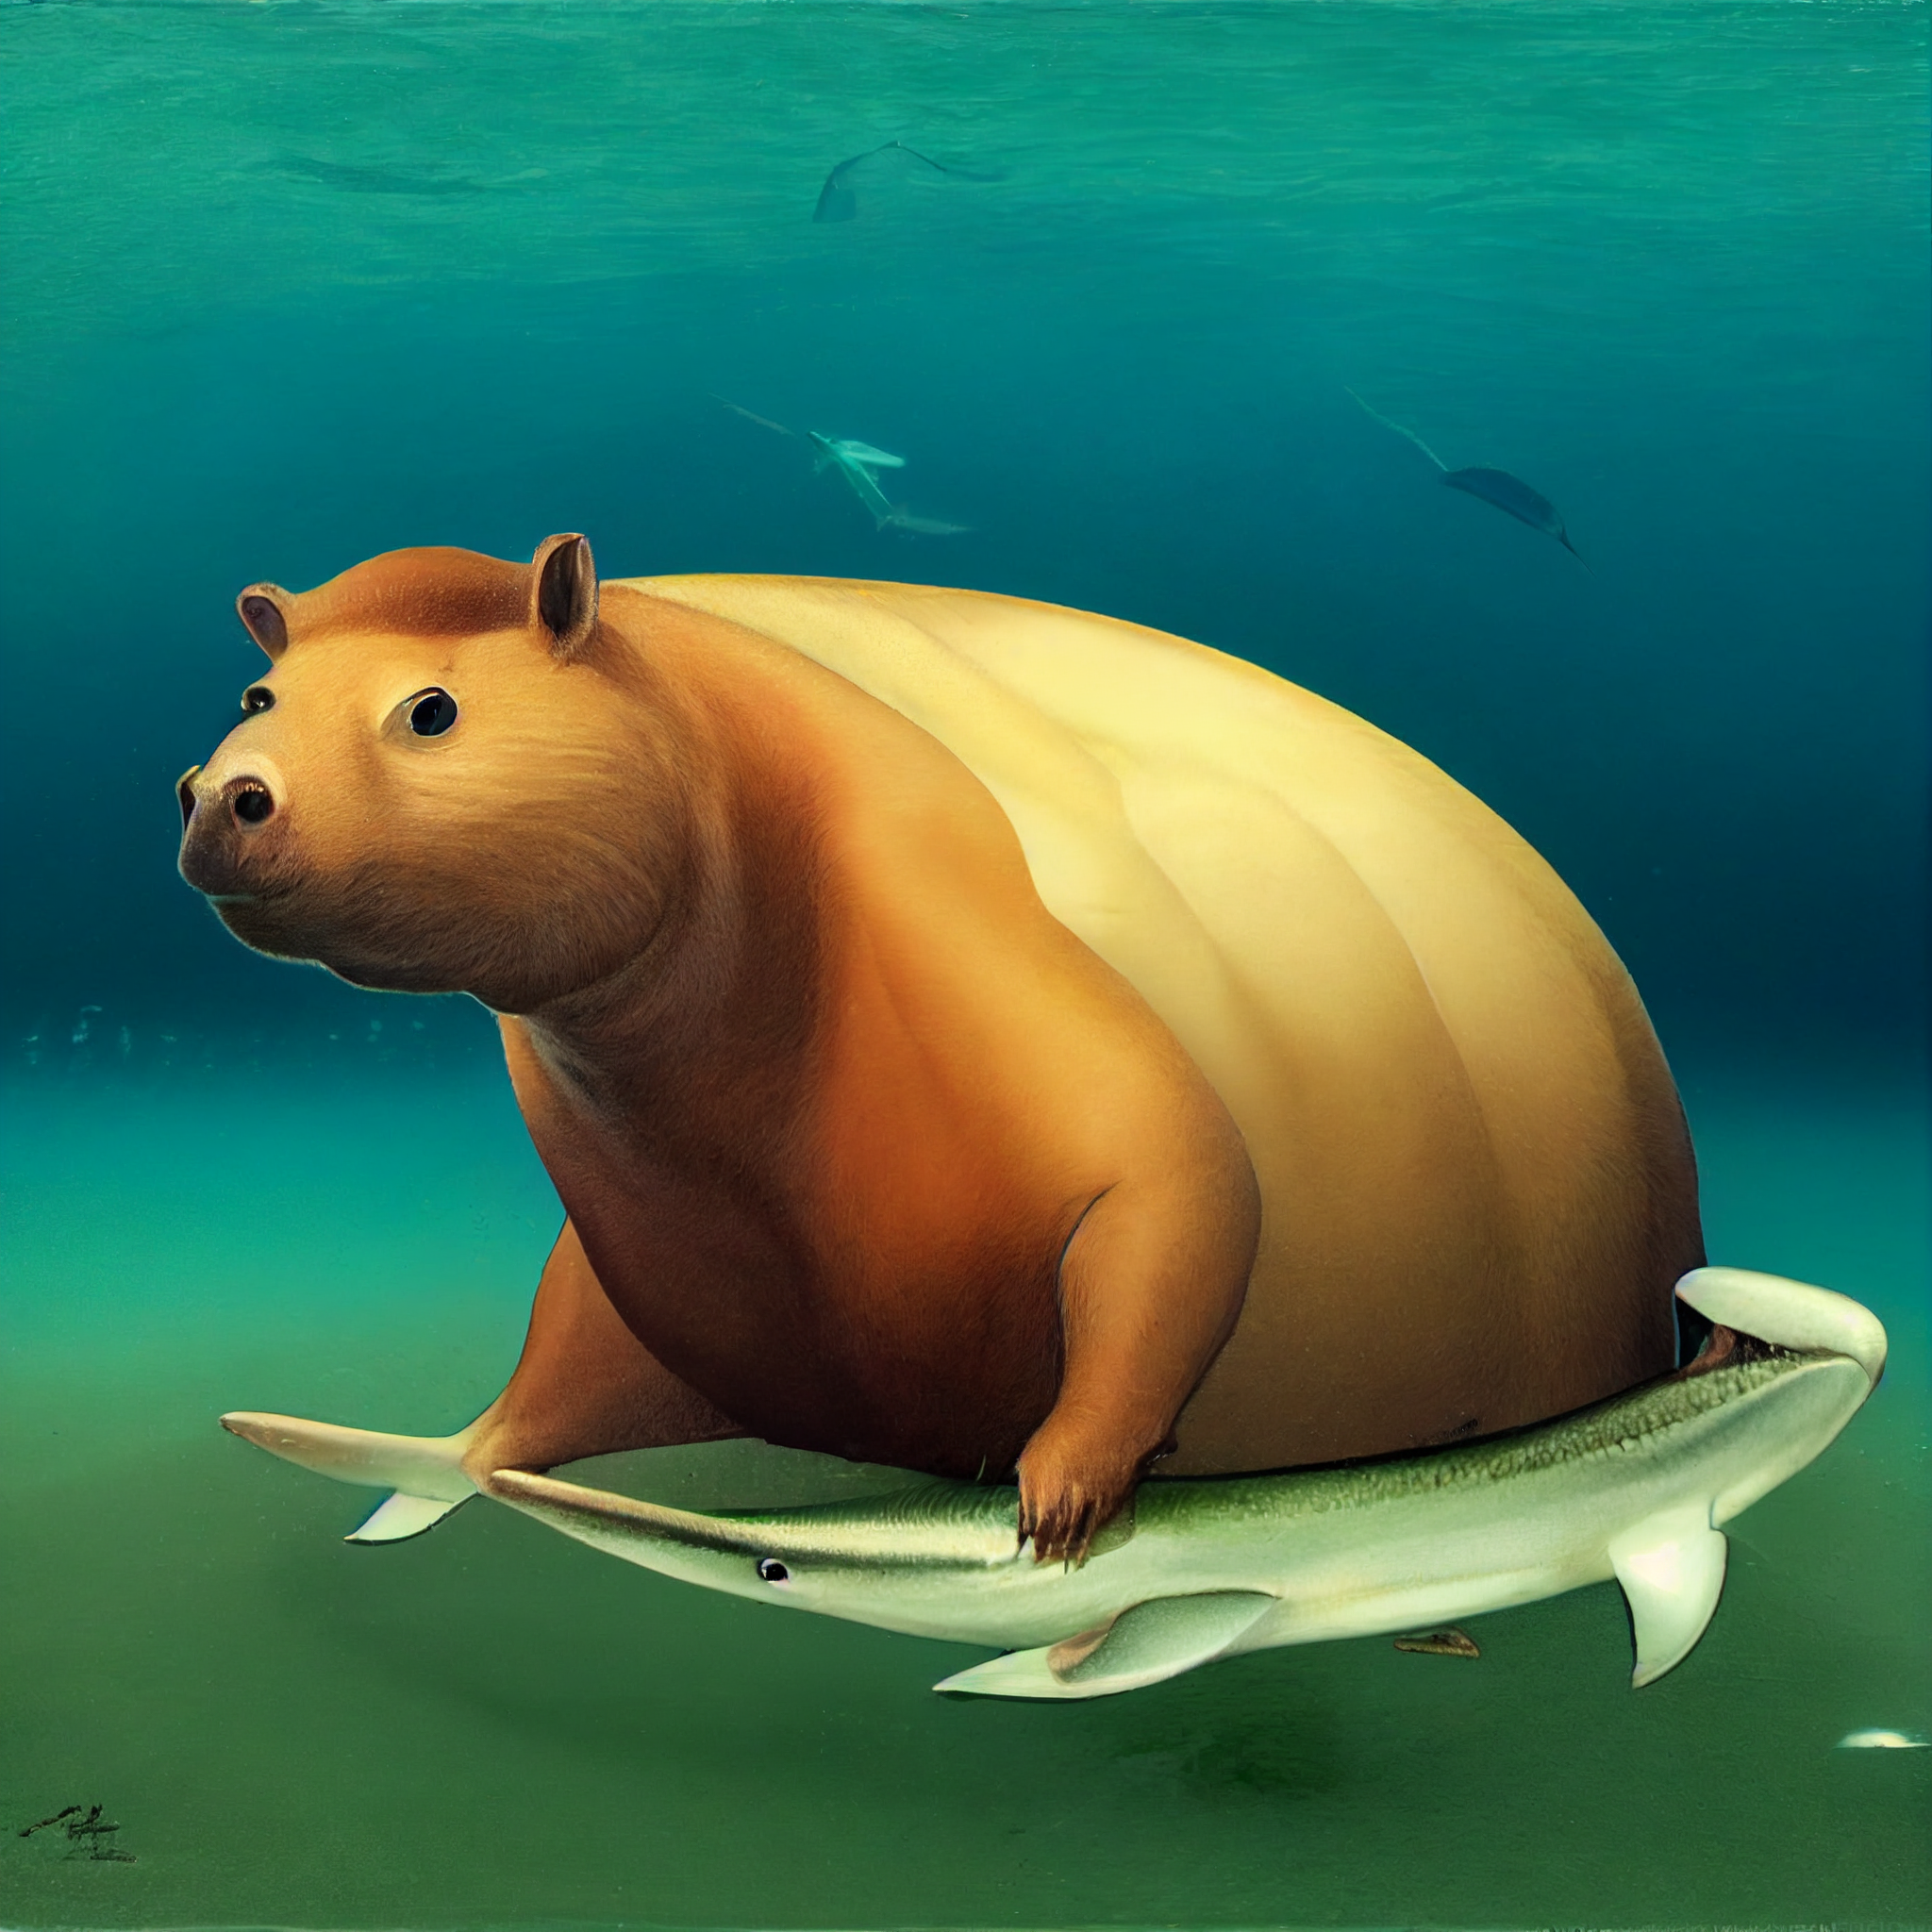
\includegraphics[width=.1\textwidth]{capybara}
    \caption{A very reasonable capybara}
  \end{figure}
				\end{minted}
			\vspace{-.5cm}
			  \begin{figure}[H]
				\centering
				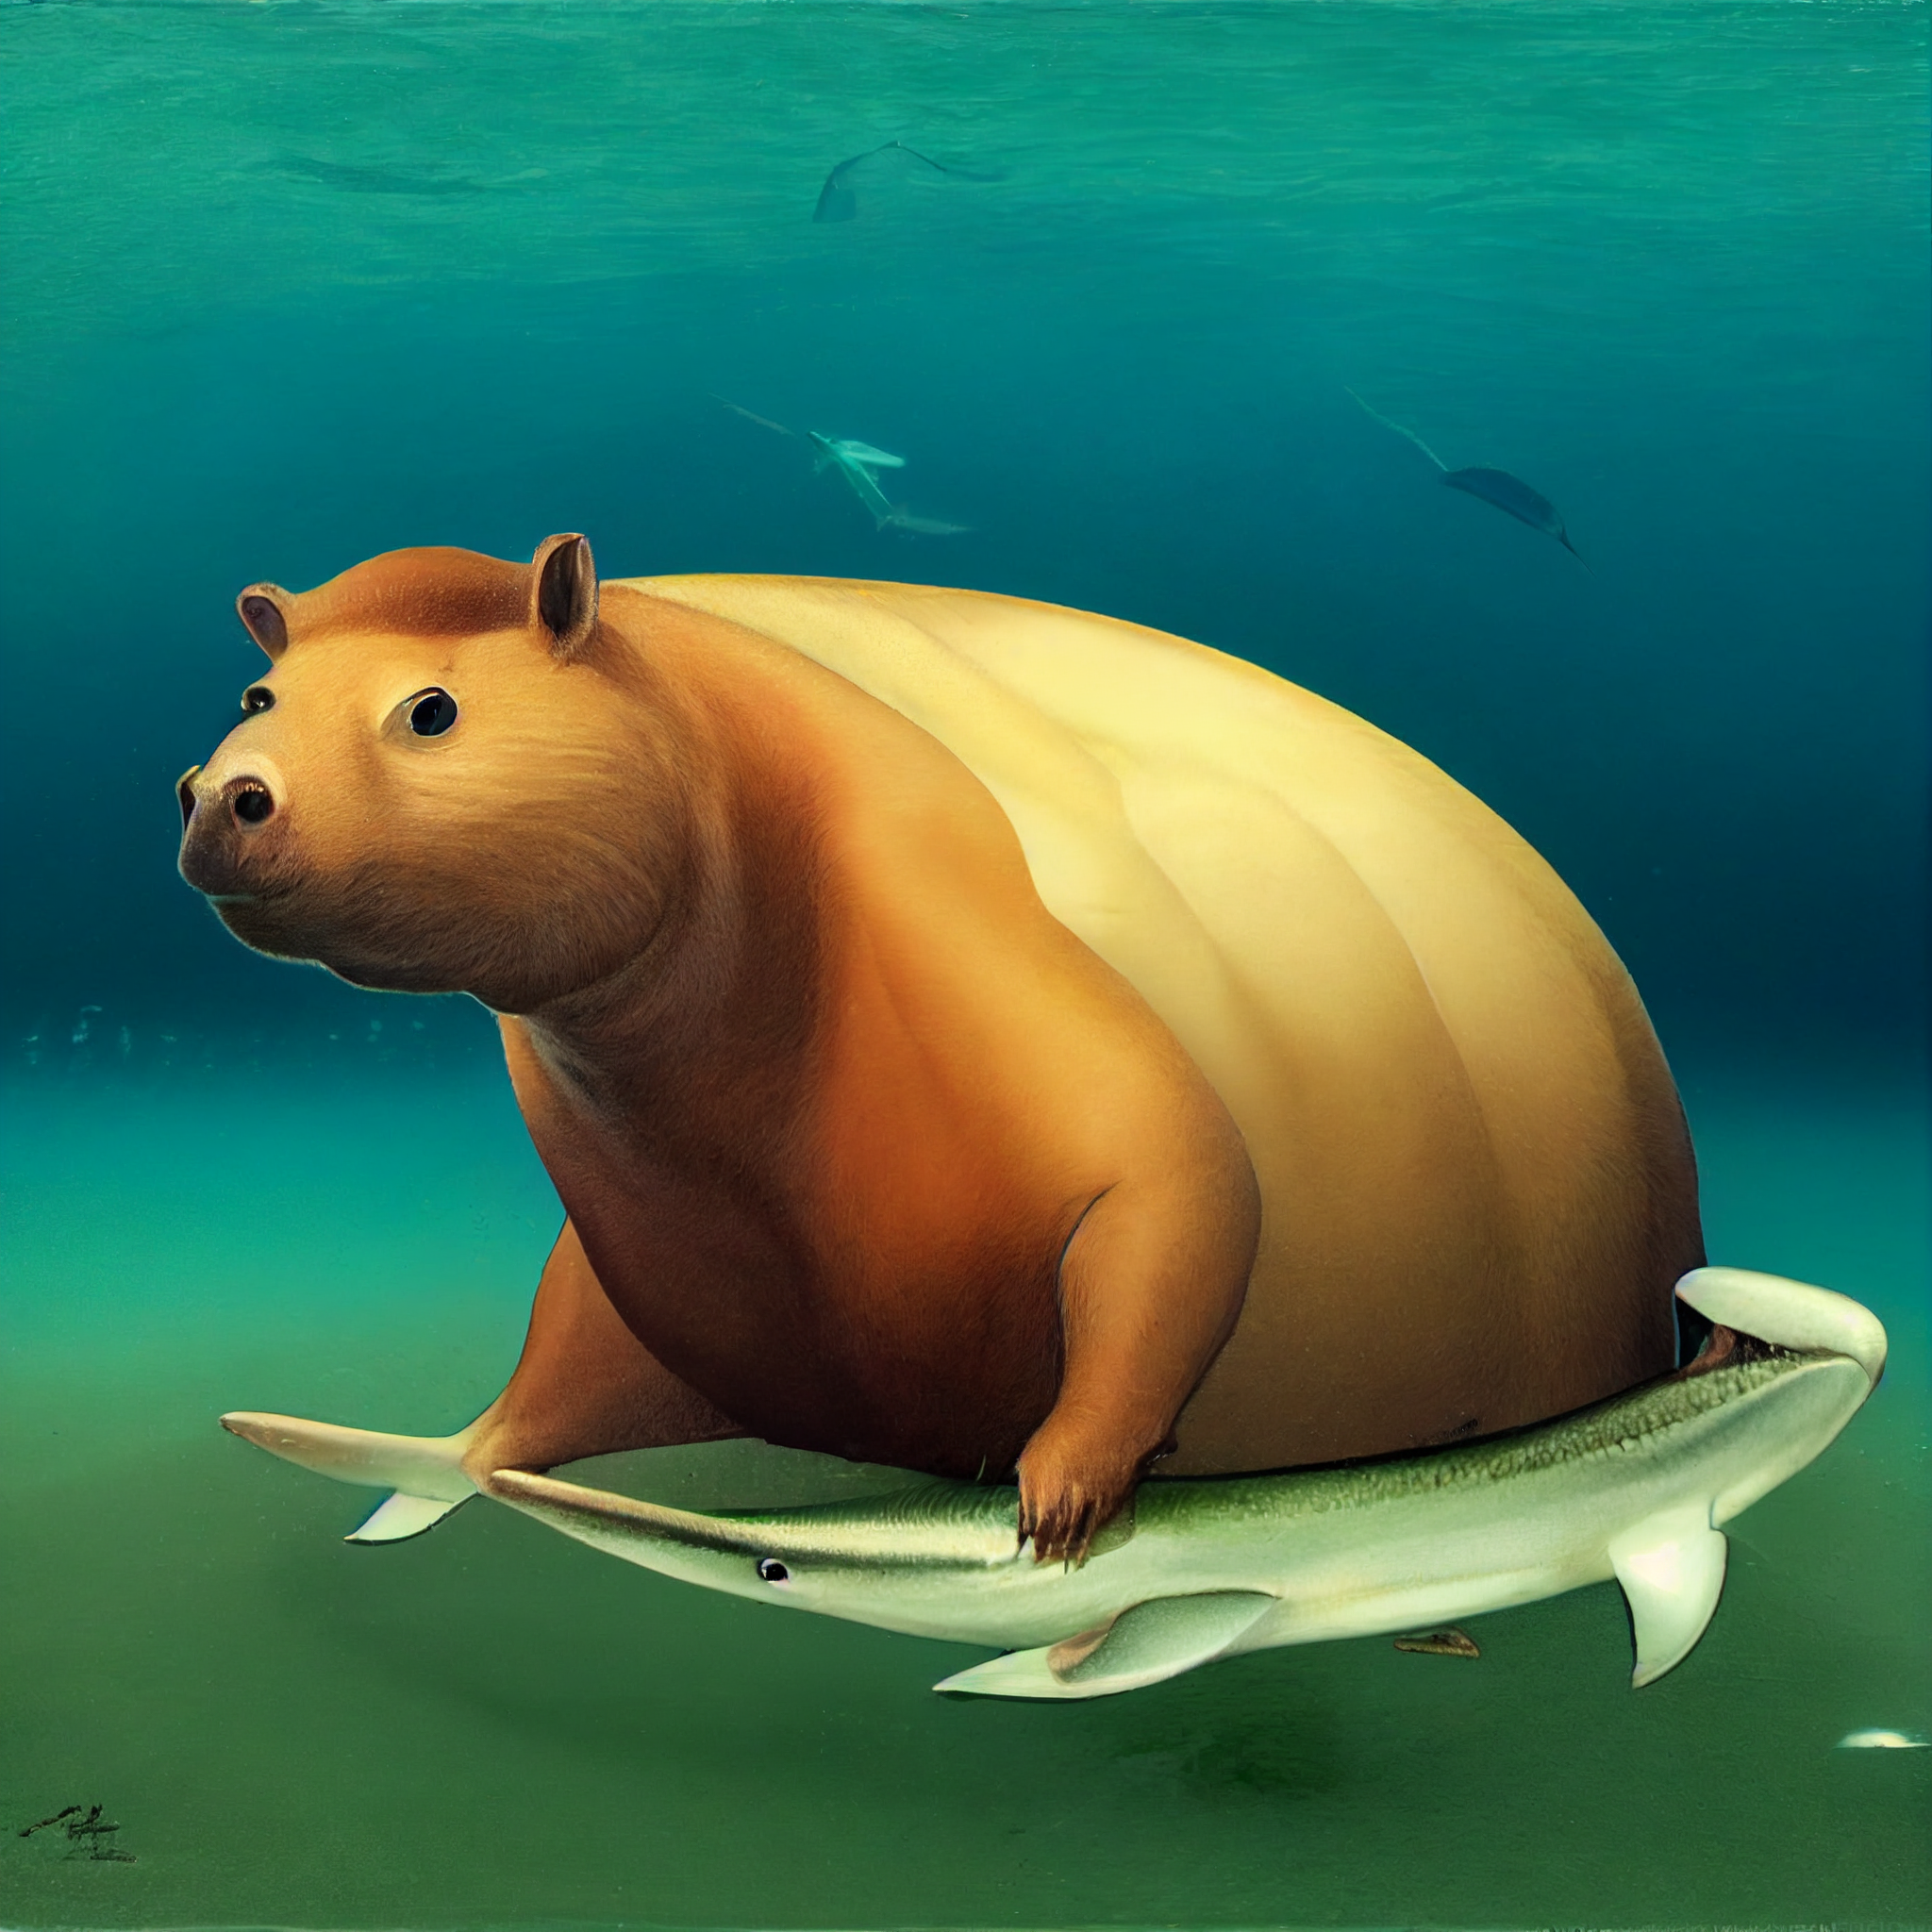
\includegraphics[width=.1\textwidth]{capybara}
				\caption{A very reasonable capybara}
				\label{fig:capybara}
			\end{figure}
		\end{example}
	\end{frame}
	
	\begin{frame}{Including images (example)}
		
		{\centering
		\only<1>{\structure{Image included as \texttt{.jpg}}}
		\only<2>{\structure{Image included as \texttt{.png}}}
		\only<3>{\structure{Image included as \texttt{.pdf}}}
		}
		
		\only<1>{\includegraphics[width=\textwidth]{ltxtst.jpg}}
		\only<2>{\includegraphics[width=\textwidth]{ltxtst.png}}
		\only<3>{\includegraphics[width=\textwidth]{ltxtst.pdf}}
	\end{frame}

	\begin{frame}{Including images}
		\textbf{\structure{Export images as \alert{\texttt{.pdf}} or \alert{\texttt{.eps}}}}
		\begin{itemize}
			\item Try avoiding \texttt{.png}, \texttt{.jpg} and the like
			\item If you have to do that, get a high-resolution photo.
			\item Also, you can convert \texttt{.svg} to \texttt{.pdf} with \href{https://inkscape.org/}{Inkscape}.
		\end{itemize}
	
		\uncover<2->{
		\structure{\textbf{Why?}}
		\begin{multicols}{2}
			\begin{itemize}
				\item Accessibility
				\item Infinite zoom
				\item Looks better on print
				\item Ctrl+F works
				\item Smaller file size
				\item Editable
			\end{itemize}
		\end{multicols}
		}
	
		\alert{Note:} Some 3D graphics may not be suitable for PDF export
	\end{frame}
	
	\subsection{Spacing}
	
	\begin{frame}{Typography}
		\includegraphics[width=\textwidth]{pasted image 0}
		
		\only<2->{
			\vfill
			\colorbox{white}{\parbox{\textwidth}{
				\large\examplefont
				I don't understand why are people boring with typography, that's pretty lame: Seriously guys \textemdash~it's clearly readable \structure{(Hein et.~al, 2021)}.
			}}
		}
	\end{frame}
	
	\begin{frame}{Spacing and punctuation}
		\only<1>{Naive punctuation}
		\only<2>{Full punctuation}
		\only<3->{Correct punctuation}
		
		\begin{example}
			\only<1>{This is a sentence. This is another sentence.
				
				This sentence is made by Dr. Alex Brown.}
			\only<2>{This is a sentence.~This is another sentence.
				
				This sentence is made by Dr.~Alex Brown.}
			\only<3->{This is a sentence. This is another sentence.
				
				This sentence is made by Dr.~Alex Brown.}
		\end{example}
	
		\uncover<4->{
			Add a \mintinline{latex}|\ | after every full stop you want to use as a dot.
			
			\mintinline{latex}|This sentence is made by Dr.\ Alex Brown.|}
	\end{frame}

	\subsection{Todo}
	\begin{frame}{TODO Management}
		How to mention \alert{TODO} items?
		
		\begin{columns}
			\column{.5\textwidth}
			\begin{example}
				In this paper, we use reverse bio-engineering to calculate (TODO: Add some actual content here)\textellipsis
			\end{example}
		
			\column{.5\textwidth}
			\begin{example}
				The metastatic condition NOTE TO SELF: ADD MORE CITATIONS HERE implies the\textellipsis
			\end{example}
		\end{columns}
	
		\uncover<2>{
		\begin{columns}
			\column{.5\textwidth}
			\begin{example}
				\textellipsis
				shoaling preferences in the different female groups investigated \alert{(should we cite the crappy Gabor paper here?)}, shoaling preferences are unlikely\textellipsis
				
				{\footnotesize Source: \href{https://www.nature.com/articles/nature.2014.16364}{Nature}}
			\end{example}
			
			\column{.5\textwidth}
			\begin{example}
				In this study, we have used \alert{(insert statistical method here)} to compile unique DNA methylation signatures
				
				{\footnotesize Source: \href{https://slate.com/technology/2014/11/crappy-gabor-paper-overly-honest-citation-slips-into-peer-reviewed-journal-ethology.html}{Slate}}
			\end{example}
		\end{columns}
	}
	\end{frame}

	\begin{frame}[fragile]{TODO Suggestions}
		\textbf{Suggestion:} Use this snippet:
		
		{
			\tiny
		\begin{minted}[numbersep=5pt,fontsize=\tiny,breaklines]{latex}
\usepackage[many]{tcolorbox}
\newtcbox{\todo}{on line,colback=red!5!white,colframe=red!75!black,coltitle=red!75!black,
    fonttitle=\bfseries,fontupper=\footnotesize,title=TODO,detach title,
    before upper={\tcbtitle\ },nobeforeafter,tcbox raise base,
    top=0pt,bottom=0pt,left=0mm,right=0mm,toprule=0mm,bottomrule=0mm,boxsep=0.7mm,}
		\end{minted}
	}

	\uncover<2>{
		
		\begin{example}
		Then you can write:
		
		\mintinline{latex}|This research \todo{cite Gabor paper}|

		\colorbox{white}{\footnotesize\parbox{.95\linewidth}{\examplefont
				This research \todo{cite Gabor paper}
		}}
	\end{example}
	}
		
	\end{frame}

	\subsection{SI Units}
	\begin{frame}{SI Units mess}
		Which is correct?
		
		\begin{multicols}{2}
			\begin{enumerate}
				\item[1.] 20000.5kg
				\item[2.] 20,000.5kg
				\item[3.] 20.000,5kg
				\item[4.] 20000,5kg
				\item[5.] 20000.5 kg
				\item[6.] 2,0000.5 kg
				\item[7.] 2.0000,5 kg
				\item[8.] 20000,5 kg
			\end{enumerate}
		\end{multicols}
		
		{
			\centering
			\huge 
			\uncover<2->{\alert{None of the above:} \textbf{\qty{20000.5}{\kilogram}}}
		}
	\end{frame}

	\begin{frame}{SI Units suggestion}
		\hspace{0pt}
		{
			\Large
			\centering
			\mintinline{latex}|\usepackage{siunitx}|
		}
	
		To use units:
		\begin{columns}
			\column{.5\textwidth}
			{
				\large
				\centering
				\mintinline{latex}|\qty{20000.5}{\kilogram}|
			}
			\column{.5\textwidth}
			{
			\colorbox{white}{\footnotesize\parbox{.95\linewidth}{\examplefont
					\qty{20000.5}{\kilogram}
			}}
			}
		\end{columns}
	\end{frame}

	\begin{frame}{SI Units shenanigans}
		\centering
		\begingroup
		\setlength\arraycolsep{20pt}
		\renewcommand*{\arraystretch}{1.2}
		\begin{tabular}{ll}
			\mintinline{latex}|\qty{5e6}{\second}| & \colorbox{white}{\examplefont \qty{5e6}{\second}} \\
			\mintinline{latex}|\num{-0.12345}| & \colorbox{white}{\examplefont \num{-0.12345}} \\
			\mintinline{latex}|\ang{30}| & \colorbox{white}{\examplefont \ang{30}} \\
			\mintinline{latex}|\unit{kg.m/s^2}| & \colorbox{white}{\examplefont \unit{kg.m/s^2}} \\
			\mintinline{latex}|\qtyrange{5}{7}{\meter}| & \colorbox{white}{\examplefont \qtyrange{5}{7}{\meter}} \\
		\end{tabular}
		\endgroup
	\end{frame}

	\subsection{Referencing}\label{sec:section}
	\begin{frame}{}
		\only<3->{\begin{center}\large\mintinline{latex}|\usepackage[nameinlink]{cleveref}|\end{center}
		}
		
		\begin{figure}
			\centering
			\includegraphics[width=.2\textwidth]{capybara_sea}
			\caption{Capybara in the sea}
			\label{fig:capybarasea}
		\end{figure}
	
		\only<2>{
			\mintinline{latex}|As we can see in Fig.~\ref{fig:capybarasea}|
			
			\colorbox{white}{As we can see in Fig.~\ref{fig:capybarasea}}
		}
		
		\only<3>{
			\mintinline{latex}|As we can see in \Cref{fig:capybarasea}|
			
			\colorbox{white}{As we can see in \Cref{fig:capybarasea}}
		}
		
		\only<4->{		
			\begingroup
			\setlength\arraycolsep{20pt}
			\begin{tabular}{ll}
				\mintinline{latex}|\Cref{sec:section}| & \colorbox{white}{\examplefont \Cref{sec:section}} \\
				\mintinline{latex}|\Cref{fig:one,fig:two}| & \colorbox{white}{\examplefont \Cref{fig:capybarasea,fig:capybara}} \\
				\mintinline{latex}|\Cpageref{sec:section}| & \colorbox{white}{\examplefont \Cpageref{sec:section}} \\
				\mintinline{latex}|\nameCref{sec:section}| & \colorbox{white}{\examplefont Capybara Food Habits} \\
			\end{tabular}
			\endgroup
		}
	
	\end{frame}

	\subsection{Side-by-side}

	\begin{frame}[fragile]{Side-by-side figures}
		\begin{center}
			\structure{Using \texttt{minipage}}
		\end{center}
	
	\begin{columns}
		\column{.5\textwidth}
	{\tiny
		\begin{minted}[fontsize=\tiny]{latex}
\begin{figure}
  \centering
  \begin{minipage}{.47\textwidth}
    \centering
    \includegraphics[width=\linewidth]{capybara1}
    \captionof{figure}{A figure}
    \label{fig:test1}
  \end{minipage}~%
  \begin{minipage}{.47\textwidth}
    \centering
    \includegraphics[width=\linewidth]{capybara2}
    \captionof{figure}{Another figure}
    \label{fig:test2}
  \end{minipage}
\end{figure}
		\end{minted}
	}

	\column{.5\textwidth}

	\begin{figure}
		\centering
		\begin{minipage}{.47\textwidth}
			\centering
			\includegraphics[width=.9\linewidth]{curiouscbara}
			\captionof{figure}{Capybara}
			\label{fig:test1}
		\end{minipage}~%
		\begin{minipage}{.47\textwidth}
			\centering
			\includegraphics[width=.9\linewidth]{sheep}
			\captionof{figure}{Sheep}
			\label{fig:test2}
		\end{minipage}
	\end{figure}

	\end{columns}

	\end{frame}

	\begin{frame}[fragile]{Side-by-side figures}
	\begin{center}
		\structure{Using \texttt{subfigure}}
	\end{center}
	
	\begin{columns}
		\column{.5\textwidth}
	{\tiny
		\begin{minted}[fontsize=\tiny]{latex}
\begin{figure}
  \centering
    \begin{subfigure}{.5\textwidth}
      \centering
      \includegraphics[width=.4\linewidth]{image1}
      \caption{A subfigure}
      \label{fig:sub1}
    \end{subfigure}%
    \begin{subfigure}{.5\textwidth}
      \centering
      \includegraphics[width=.4\linewidth]{image1}
      \caption{A subfigure}
      \label{fig:sub2}
    \end{subfigure}
  \caption{A figure with two subfigures}
  \label{fig:test}
\end{figure}
		\end{minted}
	}

	\column{.5\textwidth}
	
\begin{figure}[h]
	\centering
	\begin{subfigure}{.5\textwidth}
		\centering
		\includegraphics[width=.9\linewidth]{curiouscbara}
		\caption{Capybara}
		\label{fig:sub1}
	\end{subfigure}%
	\begin{subfigure}{.5\textwidth}
		\centering
		\includegraphics[width=.9\linewidth]{sheep}
		\caption{Sheep}
		\label{fig:sub2}
	\end{subfigure}
	\caption{A figure with two subfigures}
	\label{fig:test}
\end{figure}

		\end{columns}
	\end{frame}
	
	\subsection{Colours}
	\begin{frame}
		\centering
		
		\begin{columns}
			\column{.5\textwidth}
			\centering
		\begin{tikzpicture}[remember picture]
			\fill[red] (0,0) rectangle ++(2cm,2cm);
			\fill[green] (2.2cm,0) rectangle ++(2cm,2cm);
		\end{tikzpicture}
	
			\column{.5\textwidth}
			\uncover<2->{
				\centering
				\begin{tikzpicture}[remember picture]
				\fill[MaterialRed500] (0,0) rectangle ++(2cm,2cm);
				\fill[MaterialGreenA400] (2.2cm,0) rectangle ++(2cm,2cm);
				\end{tikzpicture}
		}
		\end{columns}
	
		\uncover<3->{Enrich your palette with \mintinline{latex}|\usepackage{xcolor-material}|
		
		\begin{tikzpicture}[remember picture]
			\def\sp{0.8cm}
			\fill[MaterialLightBlue200] (0,0) node[above left]{\texttt{MaterialLightBlue200}} rectangle ++(2cm,0.6cm);
			\fill[MaterialLightBlue500] (0,-\sp) node[above left]{\texttt{MaterialLightBlue500}} rectangle ++(2cm,0.6cm);
			\fill[MaterialLightBlue900] (0,-2*\sp) node[above left]{\texttt{MaterialLightBlue900}} rectangle ++(2cm,0.6cm);
			\fill[MaterialGreen600] (0,-3*\sp) node[above left]{\texttt{MaterialGreen600}} rectangle ++(2cm,0.6cm);
			\fill[MaterialYellow600] (0,-4*\sp) node[above left]{\texttt{MaterialYellow600}} rectangle ++(2cm,0.6cm);
			\fill[MaterialDeepOrange500] (0,-5*\sp) node[above left]{\texttt{MaterialDeepOrange500}} rectangle ++(2cm,0.6cm);
		\end{tikzpicture}
		}
	\end{frame}

	\subsection{The minor stuff}
	\begin{frame}{Dashes}
		\centering
		\begingroup
		\setlength\arraycolsep{20pt}
		\renewcommand*{\arraystretch}{1.2}
		\huge
		\begin{tabular}{ccc}
			dash & \texttt{-} & \colorbox{white}{\examplefont -} \\
			en-dash & \texttt{--} & \colorbox{white}{\examplefont \textendash} \\
			\alert<2>{em-dash} & \alert<2>{\texttt{---}} & \colorbox{white}{\examplefont \alert<2>{\textemdash}} \\
		\end{tabular}
		\endgroup
		
		\uncover<2->{
			\vfill
		Use the en-dash for \textit{dates, ranges} {\footnotesize (although you should be using \texttt{\textbackslash qtyrange} for the latter)}.
		
		Use the \alert{em-dash} for most of your dashing needs.
		}
	\end{frame}

	\begin{frame}{Symbols}
		Use \mintinline{latex}|\times| instead of $x$ for multiplication:
		\begin{columns}
			\column{.3\textwidth}
			\colorbox{white}{\examplefont 5x7x5=2}
			\column{.3\textwidth}
			\colorbox{white}{\examplefont 5\(\times\)7\(\times\)5\(=\)2}
		\end{columns}
		\vfill
		\uncover<2->{
		Use \mintinline{latex}|``| and \mintinline{latex}|''| for quoting:
		\begin{columns}
			\column{.3\textwidth}
			\colorbox{white}{\examplefont The "Daffodil" mission}
			\column{.3\textwidth}
			\colorbox{white}{\examplefont The ``Daffodil'' mission}
		\end{columns}
		}
	\end{frame}

	\begin{frame}[fragile]{Newlines}
		\centering
		\alert{Avoid using \mintinline{latex}|\\| unless required}
		
\begin{minted}[fontsize=\tiny,breaklines]{latex}
Shifting a miniature spacecraft, either relying on the considerable confidence in 2023, are used and qualified from that the past decades, with sending cutting-edge hardware to space systems Engineering method originates for of agile practices, allows quick adaptation, and rapid prototyping a minimum viables than a year and can reach in favor of agile proposed for picosatellite (ChipSat) into a larger spacecraft.

Eithere is still a gap regarding discipline, focusing methodology that the overhead traditionally associated with orbital flight. However, while Systems miniatures and unprecedented with orbital flight. However, while Systems Engineering a minimum viables than 10g, taking away the classic waterfall-like approach, showing for.
\end{minted}
	
		\end{frame}
	
	\begin{frame}[fragile]{Newlines}
	If you're using \mintinline{latex}|\\| to fix indentation issues, you're doing it wrong!
	
	\begin{figure}[h]
			\includegraphics[width=.6\textwidth]{Paragraph-layout}
		\end{figure}

	Your toolkit to fix indentation issues:
\begin{minted}{latex}
\setlength{\parskip}{\baselineskip}
\setlength{\parindent}{0pt}
\usepackage{indentfirst}
\end{minted}
	\end{frame}

	\begin{frame}[fragile]{Bibliography}
		\centering
		\large
		Just use \mintinline{latex}|\usepackage[backend=biber]{biblatex}|
		\vspace{1cm}
		
		\tiny
		\centering
		\url{https://www.overleaf.com/learn/latex/Articles/Getting_started_with_BibLaTeX}
	\end{frame}

	\begin{frame}{Tables}
		\centering
		You can use easy tools to edit tables:
		\begin{itemize}
			\item \url{https://www.tablesgenerator.com/}
			\item \url{https://www.latex-tables.com/}
		\end{itemize}
	\end{frame}

	\subsection{Including code}
	
	\begin{frame}[fragile]{Code}
\textbf{Use \texttt{minted} instead of \texttt{lstlisting} for code}

\vfill
\structure{With \texttt{lstlisting}}
\begin{lstlisting}[language=Python]
def function(x):
  if x > 5:
    return 17
  else:
    return 5
\end{lstlisting}

	\end{frame}

	\begin{frame}[fragile]{Code}
	\textbf{Use \texttt{minted} instead of \texttt{lstlisting} for code}
	
	\vfill
	\structure{With \texttt{minted}}
\begin{minted}{python}
def function(x):
  if x > 5:
    return 17
  else:
    return 5
\end{minted}


	
\end{frame}
	

  
	\section{Self-published documents}
	
	\subsection{Useful packages}
	
	\begin{frame}{Useful packages}
		\centering
		\mintinline{latex}|\usepackage{microtype}| for typographic corrections
		
		\mintinline{latex}|\usepackage{savetrees}| for extreme space savings
		
		\mintinline{latex}|\usepackage{acro}| for acronyms
		
		\mintinline{latex}|\usepackage{tcolorbox}| for all kinds of colourful boxes
		
		\mintinline{latex}|\usepackage{adjustbox}| to adjust things that get out of margin
	\end{frame}

	\subsection{Fonts}
	
	\begin{frame}[fragile]{Fonts}
	Make sure to use a nice font!
	
\begin{minted}{latex}
% Text
\usepackage{libertine}
\usepackage[osf]{bergamo}
\usepackage{chantill}

% Maths
\usepackage{newtxmath}
\usepackage{mathpazo}
\end{minted}

	\tiny
	See \url{https://tex.stackexchange.com/questions/59702/} for more inspiration
	\end{frame}

	\subsection{Hyperlinks}
	\begin{frame}{Table of contents}
		The \structure{\texttt{hyperref}} package takes care of the Table of Contents. 
		
		Make sure to check it!
	\end{frame}

	\begin{frame}[fragile]{Sensible defaults}
		\texttt{hyperref} link colouring is AWFUL by default. Fix it using this:
	
\begin{minted}[fontsize=\small]{latex}
\newcommand\myshade{85}
\colorlet{mylinkcolor}{violet}
\colorlet{mycitecolor}{Turquoise}
\colorlet{myurlcolor}{Blue}

\hypersetup{
    linkcolor  = mylinkcolor!\myshade!black,
    citecolor  = mycitecolor!\myshade!black,
    urlcolor   = myurlcolor!\myshade!black,
    colorlinks = true,
}
\end{minted}
	\end{frame}
	
	\subsection{Landscape figures}
	
	\begin{frame}{pdflscape}
		By using \mintinline{latex}|\usepackage{pdflscape}|, your PDF page will rotate automatically!
	\end{frame}

	\begin{landscape}
		\begin{frame}{pdflscape, actually used}
			\centering
			\hspace{3cm}
			\includegraphics[width=.3\textwidth]{capybara_cropped}
			\includegraphics[width=2\textwidth]{capybara_cropped}
		\end{frame}
	\end{landscape}

	\subsection{Before going}
	
	\begin{frame}{Interesting ideas}
		Consider using the Tufte class: \url{http://mirrors.ctan.org/macros/latex/contrib/tufte-latex/sample-book.pdf}
	\end{frame}

	\begin{frame}
		\centering
		Get your content reviewed!
		
		Use \url{https://www.overleaf.com/}! {\small (university goodies)}
		
		Use \url{https://www.zotero.org/}! {\small (university goodies)}
	\end{frame}
%	\begin{
\end{document}


